\clearpage
\section{M-QAM Transmitter}

\begin{tcolorbox}	
	\begin{tabular}{p{2.75cm} p{0.2cm} p{10.5cm}} 	
		\textbf{Header File}   &:& m\_qam\_transmitter.h \\
		\textbf{Source File}   &:& m\_qam\_transmitter.cpp \\
        \textbf{Version}       &:& 20190403 (\emph{Lucas Leitao})\\
	\end{tabular}
\end{tcolorbox}

This block generates a MQAM optical signal. It can also output the binary sequence. A schematic representation of this block is shown in figure \ref{MQAM_transmitter_block_diagram_simple}.

\begin{figure}[h]
	\centering
	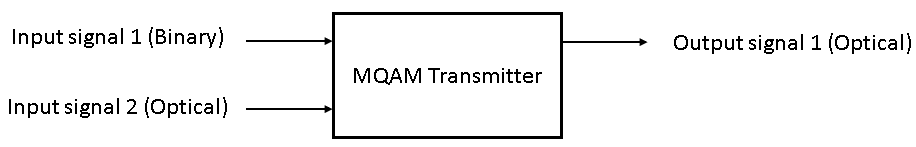
\includegraphics[width=0.6\textwidth]{./lib/m_qam_transmitter/figures/MQAM_transmitter_block_diagram_simple}
	\caption{Basic configuration of the MQAM transmitter}\label{MQAM_transmitter_block_diagram_simple}
\end{figure}

\subsection*{Functional description}

This block generates an optical signal (output signal 1 in figure \ref{MQAM_transmitter_block_diagram}). The binary signal generated in the internal block Binary Source (block B1 in figure \ref{MQAM_transmitter_block_diagram}) can be used to perform a Bit Error Rate (BER) measurement and in that sense it works as an extra output signal (output signal 2 in figure \ref{MQAM_transmitter_block_diagram}).

\begin{figure}[h]
	\centering
	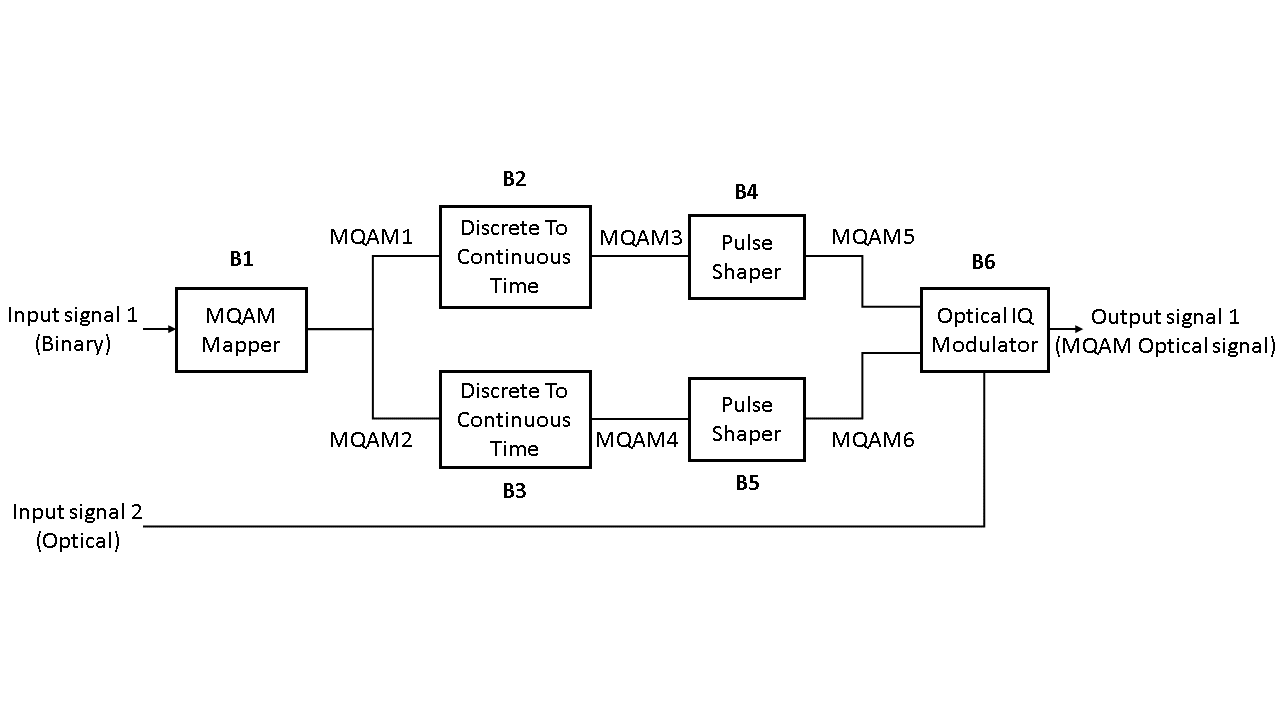
\includegraphics[width=\textwidth]{./lib/m_qam_transmitter/figures/MQAM_transmitter_block_diagram}
	\caption{Schematic representation of the block MQAM transmitter.}\label{MQAM_transmitter_block_diagram}
\end{figure}

\subsection*{Input parameters}

This block has a special set of functions that allow the user to change the basic configuration of the transmitter. The list of input parameters, functions used to change them and the values that each one can take are summarized in table \ref{table}.

\begin{table}[h]
\begin{center}
	\begin{tabular}{| m{3cm} | m{6cm} |  m{2cm} | m{4,3cm} | }
		\hline
		\textbf{Input parameters} & \textbf{Function} & Type & \textbf{Accepted values} \\ \hline
		Mode & setMode() & string & PseudoRandom \newline Random \newline DeterministicAppendZeros \newline DeterministicCyclic \\ \hline
		Number of bits generated & setNumberOfBits() & int & Any integer\\ \hline
		Pattern length & setPatternLength() & int & Real number greater than zero\\ \hline
		Number of bits & setNumberOfBits() & long & Integer number greater than zero\\ \hline
		Number of samples per symbol & setNumberOfSamplesPerSymbol() & int & Integer number of the type $2^n$ with n also integer\\ \hline
		Roll of factor & setRollOfFactor() & double & $\in$ [0,1] \\ \hline
		IQ amplitudes & setIqAmplitudes() & Vector of coordinate points in the I-Q plane & \textbf{Example} for a 4-qam mapping: \{ \{ 1.0, 1.0 \}, \{ -1.0, 1.0 \}, \{ -1.0, -1.0 \}, \{ 1.0, -1.0 \} \} \\ \hline
		Output optical power & setOutputOpticalPower() & int & Real number greater than zero\\ \hline
		Save internal signals & setSaveInternalSignals() & bool & True or False\\
		\hline
	\end{tabular}
	\caption{List of input parameters of the block MQAM transmitter} \label{table}
\end{center}
\end{table}


\pagebreak

\subsection*{Methods}

MQamTransmitter(vector$<$Signal *$>$ \&inputSignal, vector$<$Signal *$>$ \&outputSignal); (\textbf{constructor})
\bigbreak

void set(int opt);
\bigbreak
void setMode(BinarySourceMode m)
\bigbreak
BinarySourceMode const getMode(void)
\bigbreak
void setProbabilityOfZero(double pZero)
\bigbreak
double const getProbabilityOfZero(void)
\bigbreak
void setBitStream(string bStream)
\bigbreak
string const getBitStream(void)
\bigbreak
void setNumberOfBits(long int nOfBits)
\bigbreak
long int const getNumberOfBits(void)
\bigbreak
void setPatternLength(int pLength)
\bigbreak
int const getPatternLength(void)
\bigbreak
void setBitPeriod(double bPeriod)
\bigbreak
double const getBitPeriod(void)
\bigbreak
void setM(int mValue)
int const getM(void)
\bigbreak
void setIqAmplitudes(vector$<$t\textunderscore iqValues$>$ iqAmplitudesValues)
\bigbreak
vector$<$t\textunderscore iqValues$>$ const getIqAmplitudes(void)
\bigbreak
void setNumberOfSamplesPerSymbol(int n)
\bigbreak
int const getNumberOfSamplesPerSymbol(void)
\bigbreak
void setRollOffFactor(double rOffFactor)
\bigbreak
double const getRollOffFactor(void)
\bigbreak
void setSeeBeginningOfImpulseResponse(bool sBeginningOfImpulseResponse)
\bigbreak
double const getSeeBeginningOfImpulseResponse(void)
\bigbreak
void setOutputOpticalPower(t\textunderscore real outOpticalPower)
\bigbreak
t\textunderscore real const getOutputOpticalPower(void)
\bigbreak
void setOutputOpticalPower\_dBm(t\_real outOpticalPower\_dBm)
\bigbreak
t\_real const getOutputOpticalPower\_dBm(void)
\pagebreak

\subsection*{Output Signals}

\subparagraph*{Number:} 1 optical and 1 binary (optional)

\subparagraph*{Type:} Optical signal

\subsection*{Example}

%\begin{figure}[h]
%	\centering
%	\includegraphics[width=0.8\textwidth]{./lib/m_qam_transmitter/figures/BinarySource_output}
%	\caption{Example of the binary sequence generated by this block for a sequence 0100...}
%\end{figure}

%\begin{figure}[h]
%	\centering
%	\includegraphics[width=0.8\textwidth]{./lib/m_qam_transmitter/figures/IQmodulator0_output}
%	\caption{Example of the output optical signal generated by this block for a sequence 0100...}
%\end{figure}

\subsection*{Sugestions for future improvement}

Add to the system another block similar to this one in order to generate two optical signals with perpendicular polarizations. This would allow to combine the two optical signals and generate an optical signal with any type of polarization.

//%%%%%%%%%%%%%%%%%%%%%%%%%%%%%%%%%%%%%%%%%%%%%%%%%%%%%%%%%%%%%%%%%%%%%%%%%%%%%%%%%%%%%%%%%%%%%%%%%%%%%%%%%%%%%%%%%%%%%%%%%%%%%%%%%%%%%%%%%%%%%%%%%%
//%%%%%%%%%%%%%%%%%%%%%%%%%%%%%%%%%%%%%%%%%%%%%%%%%%%%%%%%%%%%%%%%%%%%%%%%%%%%%%%%%%%%%%%%%%%%%%%%%%%%%%%%%%%%%%%%%%%%%%%%%%%%%%%%%%%%%%%%%%%%%%%%%%
//%%%%%%%%%%%%%%%%%%%%%%%%%%%%%%%%%%%%%%%%%%%%%%%%%%%%%%%%%%%%%%%%%%%%%%%%%%%%%%%%%%%%%%%%%%%%%%%%%%%%%%%%%%%%%%%%%%%%%%%%%%%%%%%%%%%%%%%%%%%%%%%%%%

 \subsection*{\textbf{Version 20190403}}


This "super block" accepts a binary sequence and the local oscillator(laser) as inputs. The output is an MQAM optical signal. It can also "output" the input binary sequence (for BER calculation purposes). A schematic representation of this block is shown in figure \ref{MQAM_transmitter_block_diagram_simple}.

\begin{figure}[H]
	\centering
	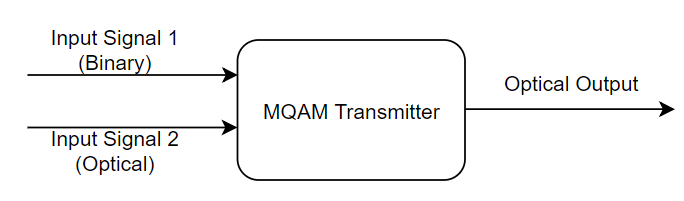
\includegraphics[width=0.6\textwidth]{./lib/m_qam_transmitter/figures/MQAM_transmitter_block_diagram_simple3}
	\caption{Basic configuration of the MQAM transmitter}\label{MQAM_transmitter_block_diagram_simple}
\end{figure}
\subsection*{Input Signals}

\subparagraph*{Number:} 1 optical and 1 binary

\subparagraph*{Type:} Optical signal and binary

\subsection*{Output Signals}

\subparagraph*{Number:} 1 optical (and 1 binary)

\subparagraph*{Type:} Optical signal (and binary sequence)

\subsection*{Input parameters}

The transmitter block has a special set of functions that allow the user to change the basic configuration of the transmitter. \\
The input parameters can be later changed by calling the "set" methods described in the next "Methods" subsection.
\begin{table}[H]
\centering
\begin{center}
	\begin{tabular}{| p{3cm} | p{5cm} | p{3cm} | p{4cm} | }
		\hline
		\textbf{Input parameters} & \textbf{Function} & Type & \textbf{Accepted values} \\ \hline
        mValue & void setM & int & Integer positive value\\
        \hline
		fTime & void setFirstTime & boolean & True or False\\
        \hline
		nSamples PerSymbol & void setNumber OfSamples PerSymbol & int & Integer number which is a power of two\\
        \hline
        iqAmplitudes Values & void setIq Amplitudes & vector<vector<t\_real>> & Vector of coordinate points in the I/Q plane \\
        \hline
        impResponse TimeLength & void setImpulse ResponseTime Length\_symbolPeriods & int & Integer positive\\
		\hline
        fType & void setFilterType & pulse\_shapper\_filter\_type  & Raised Cosine, Root Raised Cosine, Gaussian, Square\\
        \hline
        rOffFactor & void setRoll OffFactor & double & Between 0 and 1 (inclusive) \\
        \hline
        pWidth & void setPulse Width & double & Real Positive\\
        \hline
        pFilterMode & void setPassive FilterMode & boolean & True or False\\
		\hline
	\end{tabular}
	\caption{List of input parameters of the block MQAM transmitter} \label{table}
\end{center}
\end{table}
\pagebreak

\subsection*{Methods}
\begin{enumerate}
\item Block Declaration and Initialization
             \begin{itemize}
                 \item MQamTransmitter(initializer\_list$<$Signal *$>$ \&inputSig, initializer\_list$<$Signal *$>$ \&outputSig)
                 \item void initialize(void)
	             \item bool runBlock(void)
             \end{itemize}
\item Functions to set parameters
             \begin{itemize}
                \item void setM(int mValue)
                \item void setFirstTime(bool fTime)
                \item void setIqAmplitudes(vector<vector<t\_real>> iqAmplitudesValues)
                \item void setNumberOfSamplesPerSymbol(int nSamplesPerSymbol)
                \item void setImpulseResponseTimeLength\_symbolPeriods(int impResponseTimeLength)
                \item void setFilterType(pulse\_shapper\_filter\_type fType)
                \item void setRollOffFactor(double rOffFactor)
                \item void setPulseWidth(double pWidth)
                \item void setPassiveFilterMode(bool pFilterMode)
             \end{itemize}
\item Functions to get parameters
             \begin{itemize}
                \item bool getFirstTime()
                \item int const getNumberOfSamplesPerSymbol(void)
                \item int const getImpulseResponseTimeLength\_symbolPeriods(void)
                \item pulse\_shapper\_filter\_type const getFilterType(void)
                \item double const getRollOffFactor()
                \item double const getPulseWidth()
                \item bool const getPassiveFilterMode()
             \end{itemize}
\end{enumerate}

\pagebreak
\subsection*{Functional description}

The transmitter super block generates an optical signal (output signal in figure \ref{MQAM_transmitter_block_diagram}). The binary signal generated in the internal block Binary Source (block B1 in figure \ref{MQAM_transmitter_block_diagram}) can be used to perform a Bit Error Rate (BER) measurement and in that sense it works as an extra  virtual output signal.

\begin{figure}[H]
	\centering
	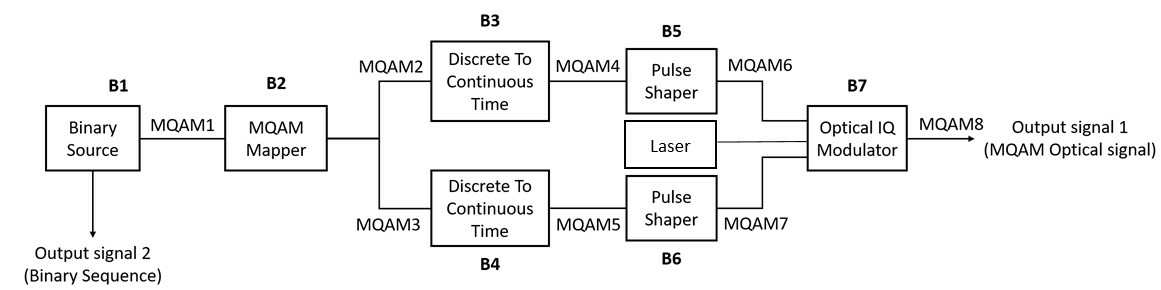
\includegraphics[width=\textwidth]{./lib/m_qam_transmitter/figures/MQAM_transmitter_block_diagram2}
	\caption{Schematic representation of the block MQAM transmitter.}\label{MQAM_transmitter_block_diagram}
\end{figure}
In a Succinct way, the transmitter maps the input binary sequence (with the M-QAM Mapper) into a constellation and then processes the resulting I/Q sinals with the "Discret-to-Continuos" and "Pulse Shaping" blocks. Both the 'I' and 'Q' signal are then optical modulated and sent to the optical channel.

\subsection*{Examples}
\subsection*{Different Coding Test}
Considering the QPSK Constellation and by adding some thermal noise ($rxThermalNoisePower=1e-3$) in the "M-QAM Receiver", we can check the effect of Gray's codification in the BER.\\
Both the Gray and normal codifications were simulated, and the BER results were then obtained:
\begin{figure}[H]
	\centering
	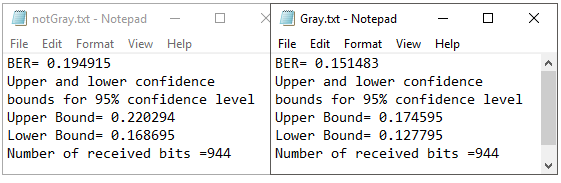
\includegraphics[scale=0.5]{./lib/m_qam_transmitter/figures/Coding}
	\caption{BER for Normal/Grey Codifications, respectively.}\label{Coding}
\end{figure}
We can conclude that the Grey codification has a minor BER (so a better system performance) because each constellation point only differs with it's neighbours by one bit (decreasing the probability of bit error).
\subsection*{Cardinality Test}
By increasing the number of the constellation points, with a thermal noise relatively high, its expected to see an increase of the BER since each constellation point has a greater probability of being decoded has one of its "neighbours".
Knowing that in advance, a simple test can be made by changing the cardinality of the transmission system from 4 to 16 (for example):
\begin{figure}[H]
	\centering
	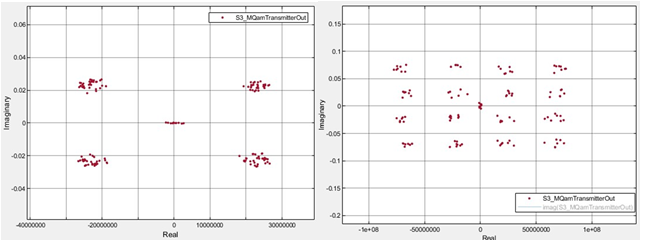
\includegraphics[scale=0.5]{./lib/m_qam_transmitter/figures/Cardinality}
	\caption{QPSK and 16QAM Constellations.}\label{Cardinality}
\end{figure}
After Changing the Input Parameters of the decoder (receiver side) to match the transmitted constellation and after adding some thermal noise, we can check the BER logs for each case:
\begin{figure}[H]
	\centering
	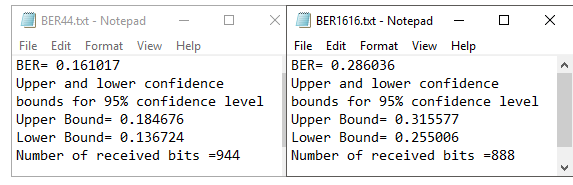
\includegraphics[scale=0.75]{./lib/m_qam_transmitter/figures/CardiBER}
	\caption{BER for QPSK and 16QAM Constellations.}\label{CardiBER}
\end{figure}
We can see that for the 16QAM constellation the BER is larger than for the QPSK case, as predicted.

\subsection*{Pulse Shaping Test}
Starting with the Pulse Shaping test, we can choose from a variety of filters. The predefined filter is the "Raised Cosine", which the following eye's diagram corresponds to:
\begin{figure}[H]
	\centering
	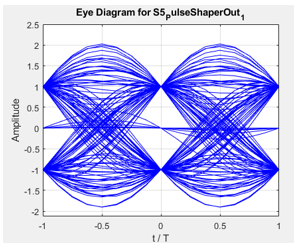
\includegraphics[scale=0.75]{./lib/m_qam_transmitter/figures/raised_01}
	\caption{ Raised Cosine Pulse Shaper Eye Diagram.}\label{raised_01}
\end{figure}
As expected, there is no ISI (Because the impulse response is zero at intervals of the symbol period). By changing the filter to "Root Raised Cosine", we can now see that some ISI will start to be visible (Because the impulse response is different than zero at intervals of the symbol optimum sampling instant).
\begin{figure}[H]
	\centering
	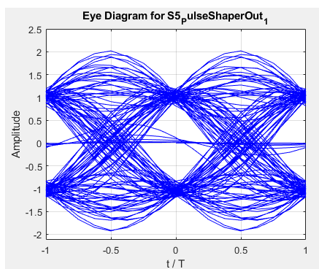
\includegraphics[scale=0.75]{./lib/m_qam_transmitter/figures/rootraised_01}
	\caption{Root Raised Cosine Pulse Shaper Eye Diagram.}\label{rootraised_01}
\end{figure}
However, this kind of filter is very useful if the electrical filter at the receiver side if it is also "Root Raised Cosine", because those same interferences will be cancelled (Since both filters form a "Raised Cosine Filter"),and the received data can be accurately decoded. (This result is visible in the Receiver Section -Examples).\\
\subsection*{Roll-Off Factor Test}
The roll-off factor (which value is between 0 and 1) is directly related to the bandwidth of the pulse shaper filter and to how fast its impulses decay. The system default value is 0.1 and in the Figure \ref{raised_01} its possible to see the consequent eye diagram.\\
By changing its value to 0.9, we can see that the correpondant eye diagram looks like a much more compact version of the previous one.
\begin{figure}[H]
	\centering
	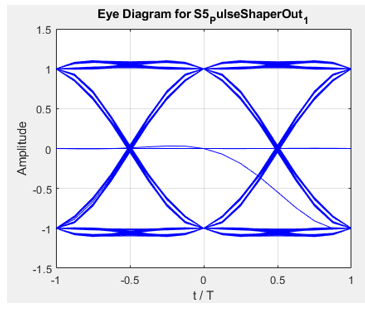
\includegraphics[scale=0.75]{./lib/m_qam_transmitter/figures/raised_09}
	\caption{Raised Cosine Pulse Shaper Eye Diagram (Rool-Off =0.9).}\label{raised_09}
\end{figure}
This happens because with a higher roll off factor, the higher the impulse decay, which originates a lower ISI when there are synchronization issues.

\subsection*{Open Issues}
\begin{itemize}
\item The "MQamMapper" setM() method only accepts two different constellations (QPSK and 16QAM).
\item The "MQamMapper" only accepts one type of codification
\item A problem with the "Vizualizer.m" makes impossible to analyse the different signal in the frequency domain\\
\end{itemize}

\subsection*{Sugestions for future improvement}
\begin{itemize}
\item Improve the Code "readability" (just by deleting unnecessary commentaries)
\item Improve the "MQamMapper" versatility, by enabling it to mapp a wider range of constellations and codifications
\item Some Block input parameters are defined in the block header file (it would be easir to simulate the system, if all system parameters were accessible in the main file).
\end{itemize}
